\documentclass[a4paper,11pt,UTF8]{article}
\usepackage{ctex}
\usepackage{amsmath,amsthm,amssymb,amsfonts}
\usepackage{amsmath}
\usepackage[a4paper]{geometry}
\usepackage{graphicx}
\usepackage{microtype}
\usepackage{siunitx}
\usepackage{booktabs}
\usepackage[colorlinks=false, pdfborder={0 0 0}]{hyperref}
\usepackage{cleveref}
\usepackage{esint} 
\usepackage{graphicx}
\usepackage{ragged2e}
\usepackage{pifont}
\usepackage{extarrows}
\usepackage{mathptmx}
\usepackage{float}
\usepackage{caption}
\usepackage{multirow}
\usepackage{subfigure}
\usepackage{titlesec}
\captionsetup[figure]{name={图}}
%opening
\title{数字电子技术作业(三)}
\author{谢悦晋 \quad U202210333}
\date{Oct 23rd, 2023 }
\begin{document}
\maketitle
\textbf{4.4.9} 试用74HC138和必要的与非门,设计一个乘法器电路,实现两位二进制数相乘,并输出结果。

解:

设输入分别为$A_1,A_0,B_1,B_0$,输出为$P_3,P_2,P_1,P_0$,列写真值表和逻辑函数:

\begin{table*}[h]
	\centering
	\caption*{4.4.9真值表}
	
	\begin{tabular}{cccc|cccc}
		\hline
		$A_1$ & $A_0$ & $B_1$ & $B_0$ & $P_3$ & $P_2$ & $P_1$ & $P_0$\\
		\hline
		0 & 0 & 0 & 0 & 0 & 0 & 0 & 0\\
		0 & 0 & 0 & 1 & 0 & 0 & 0 & 0\\
		0 & 0 & 1 & 0 & 0 & 0 & 0 & 0\\
		0 & 0 & 1 & 1 & 0 & 0 & 0 & 0\\
		0 & 1 & 0 & 0 & 0 & 0 & 0 & 0\\
		0 & 1 & 0 & 1 & 0 & 0 & 0 & 1\\
		0 & 1 & 1 & 0 & 0 & 0 & 1 & 0\\
		0 & 1 & 1 & 1 & 0 & 0 & 1 & 1\\
		1 & 0 & 0 & 0 & 0 & 0 & 0 & 0\\
		1 & 0 & 0 & 1 & 0 & 0 & 1 & 0\\
		1 & 0 & 1 & 0 & 0 & 1 & 0 & 0\\
		1 & 0 & 1 & 1 & 0 & 1 & 1 & 0\\
		1 & 1 & 0 & 0 & 0 & 0 & 0 & 0\\
		1 & 1 & 0 & 1 & 0 & 0 & 1 & 1\\
		1 & 1 & 1 & 0 & 0 & 1 & 1 & 0\\
		1 & 1 & 1 & 1 & 1 & 0 & 0 & 1\\
		\hline
	\end{tabular}
	\label{table_MAP}
\end{table*}
\begin{figure}[H]
	\centering
	\setcounter{subfigure}{0}
	\subfigure[$P_2$]{
		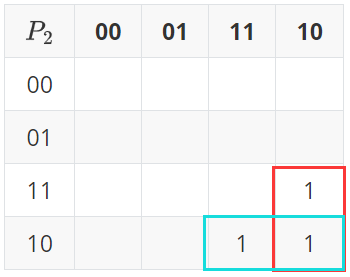
\includegraphics[width=0.3\textwidth]{4.4.9_1}
	}
	\subfigure[$P_1$]{
		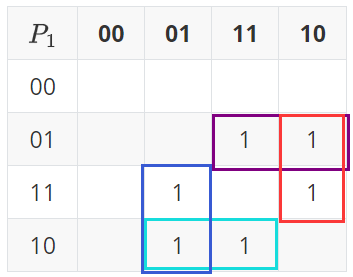
\includegraphics[width=0.3\textwidth]{4.4.9_2}
	}
	\subfigure[$P_0$]{
		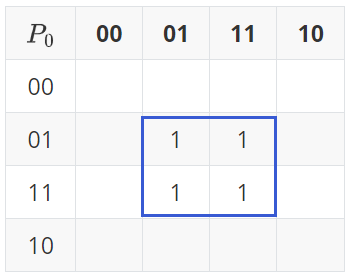
\includegraphics[width=0.3\textwidth]{4.4.9_3}
	}
	\caption{4.4.9卡诺图}
\end{figure}
$$\begin{aligned}
	P_3&=A_1A_0B_1B_0\\
	P_2&=A_1\overline{A}_0B_1+A_1B_1\overline{B}_0\\
	P_1&=A_1\overline{A}_0B_0+A\overline{B}_1B_0+A_0B_1\overline{B}_0+\overline{A}_1A_0B_1\\
	P_0&=A_0B_0
\end{aligned}
$$

\textbf{4.4.12} 图题 4.4.12 所示为 8×8 个 LED 阵列显示示意图。3 线-8 线译码器控制逐行扫描, 从上到下每次显示一行。存储阵列共有8×8 个存储单元,每个单元存放 1位显示的数据,需要显示的点存 1,否则存 0。地址线 $W_2W_1W_0$ 从 000 到 111 变化时,每次将一组 8 个数据送到输出端,控制发光二极管,需要发光的二极管接 1,否则接 0。如要显示的字形如图题 4.4.12(b)所示, 试写出存储器存放的数据。若人的视觉暂留时间为 0.05 s,在满足 LED 阵列图像稳定不闪烁的情况下,试计算地址变换的最低频率。
\begin{figure}[H]
	\centering
	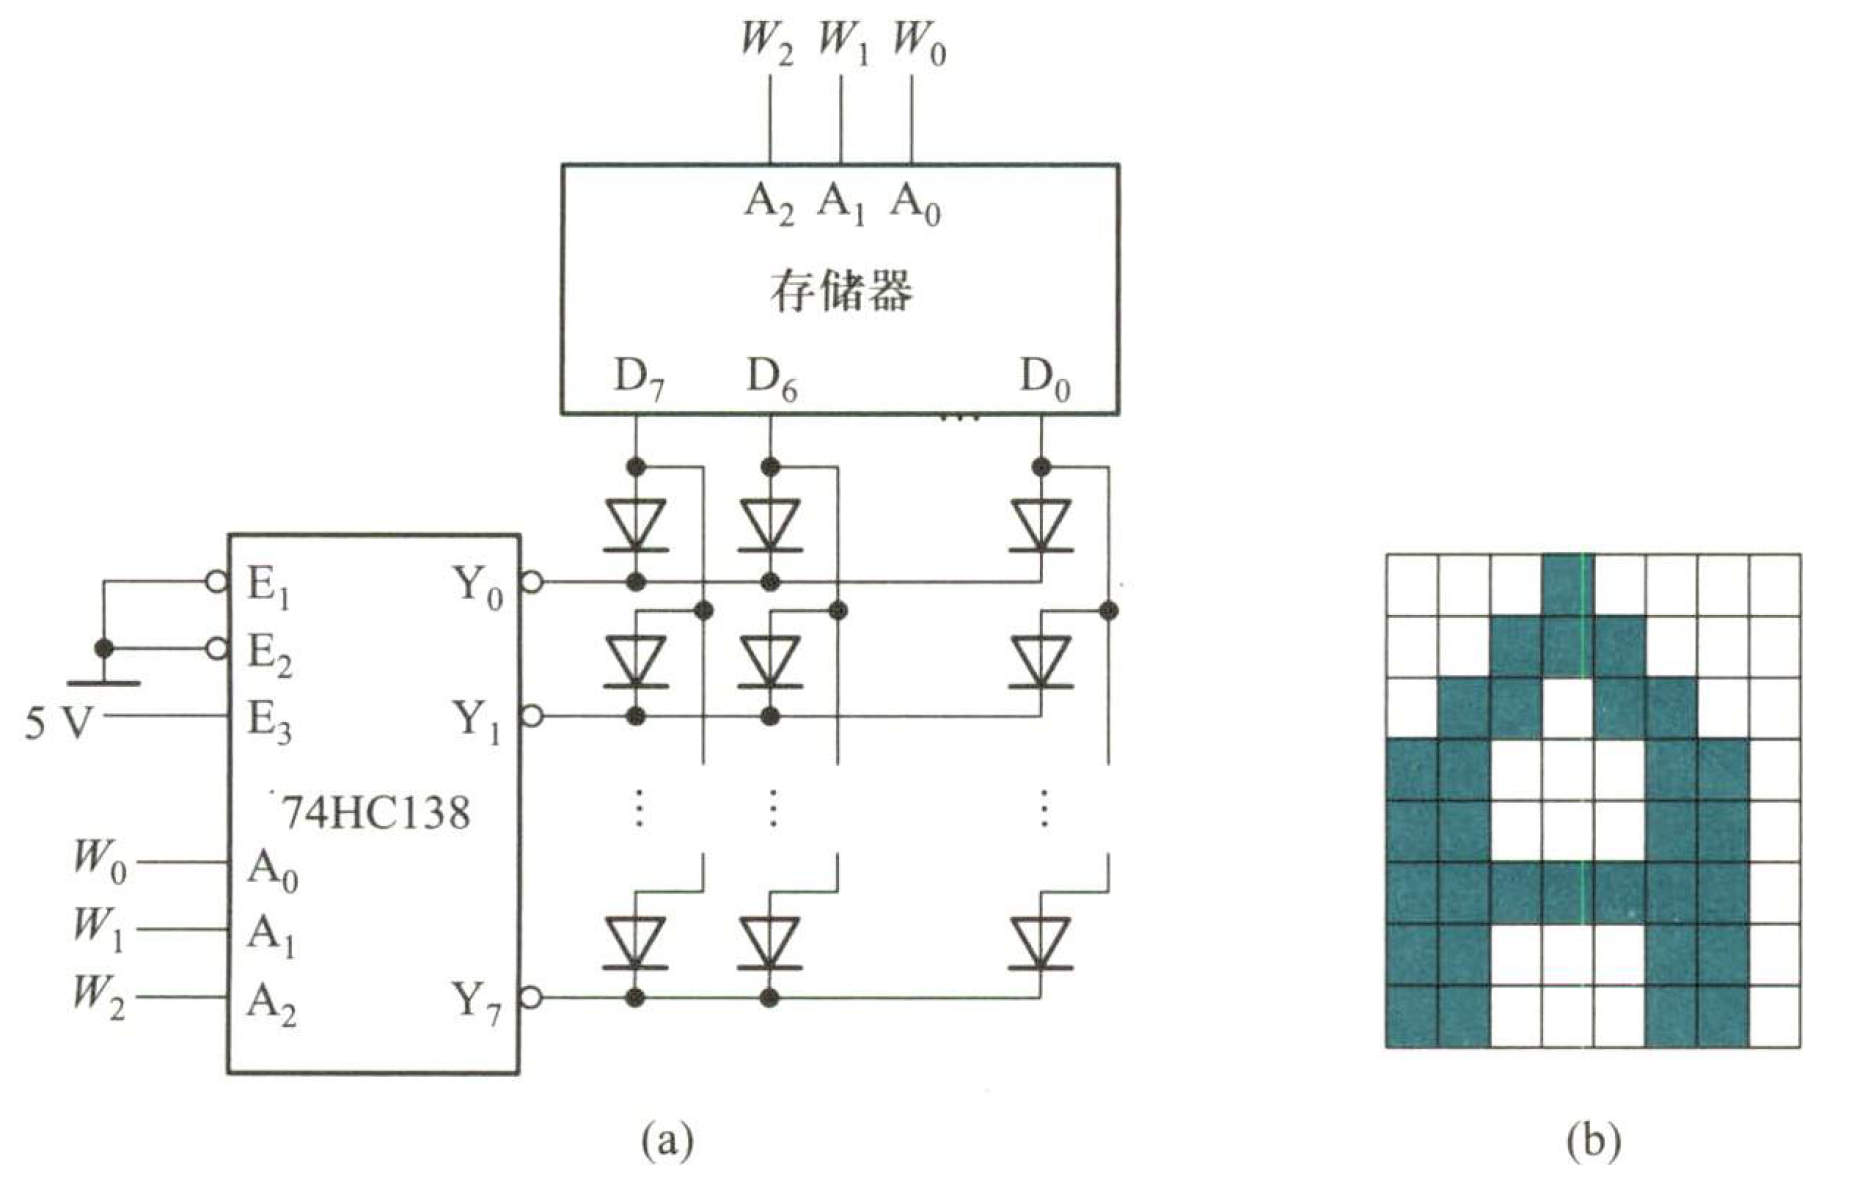
\includegraphics[width=1\textwidth]{4.4.12}
\end{figure}
解:


\textbf{4.4.20} 试用4选1数据选择器产生下列逻辑函数:

$(1)L(A,B)=\overline{A}\cdot\overline{B}+AB$

$(2)L(A,B,C)=\sum m(1,2,6,7)$

\textbf{4.4.23}具有低使能控制的8选1数据选择器(74HC151,$\overline{E}={1}$ 时,$Y={0}$)构成的电路和各输入端的输入波形如图题 4.4.23 所示,画出输出端 $Y$ 的波形。
\begin{figure}[H]
	\centering
	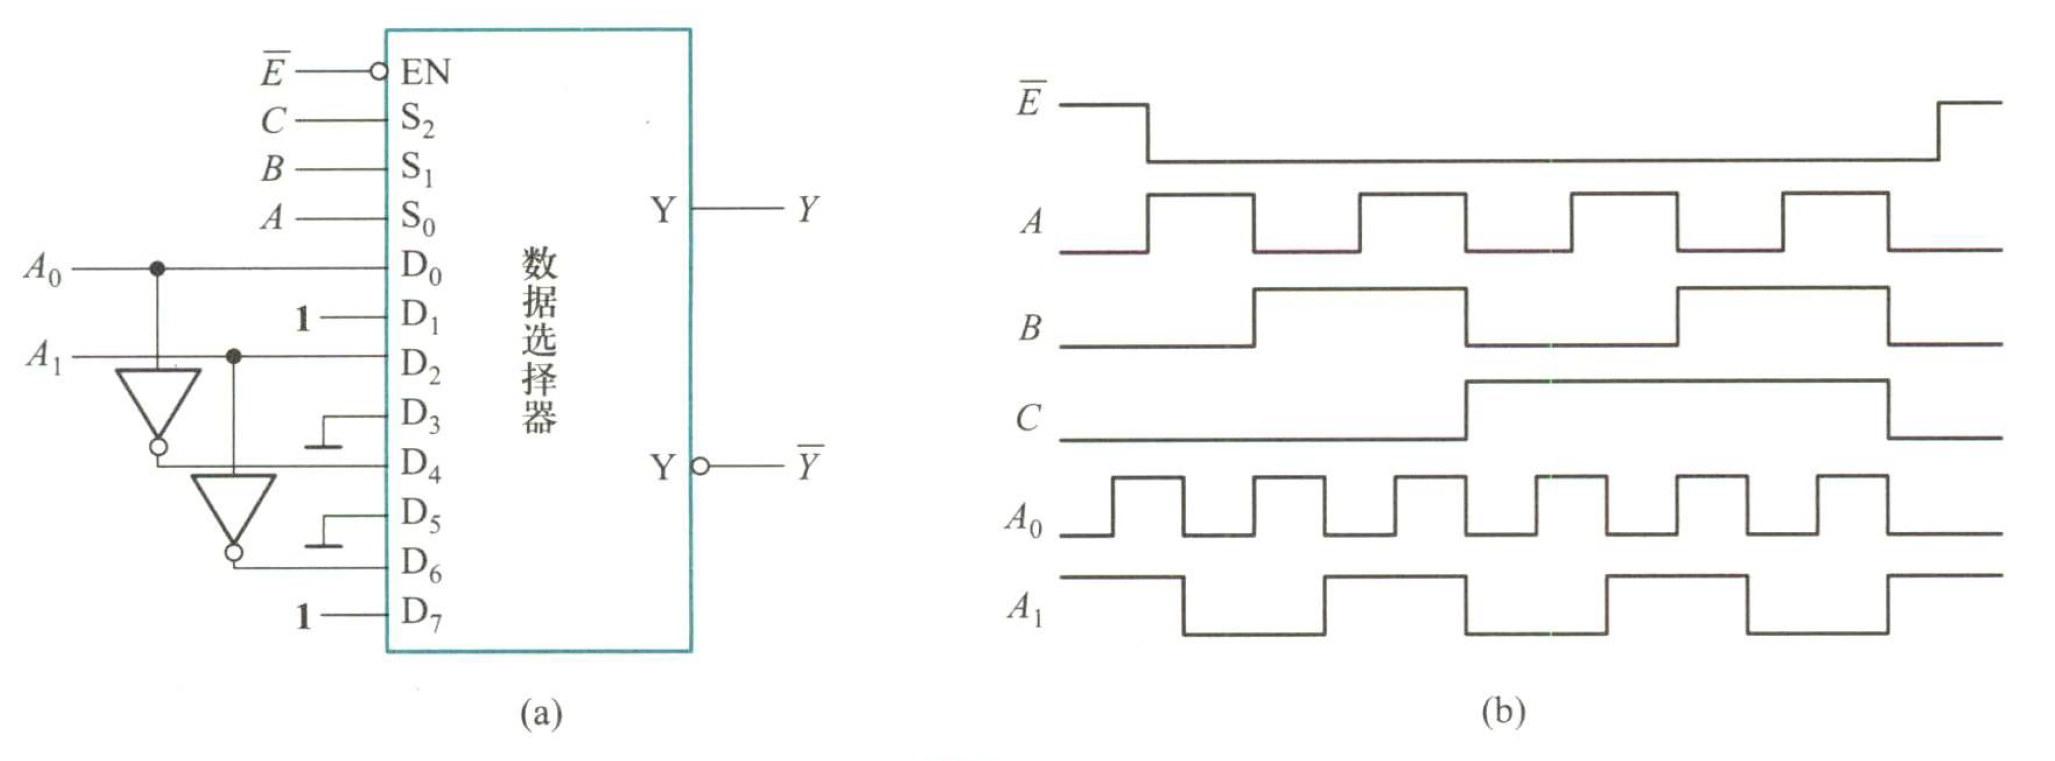
\includegraphics[width=1\textwidth]{4.4.23}
\end{figure}
\textbf{4.4.35} 仿照半加器和全加器的设计方法,试设计一半减器和一全减器,所用的门电路由自己选定。

\textbf{4.4.37} 逻辑电路如图题 4.4.37 所示,试分析该电路的功能
\begin{figure}[H]
	\centering
	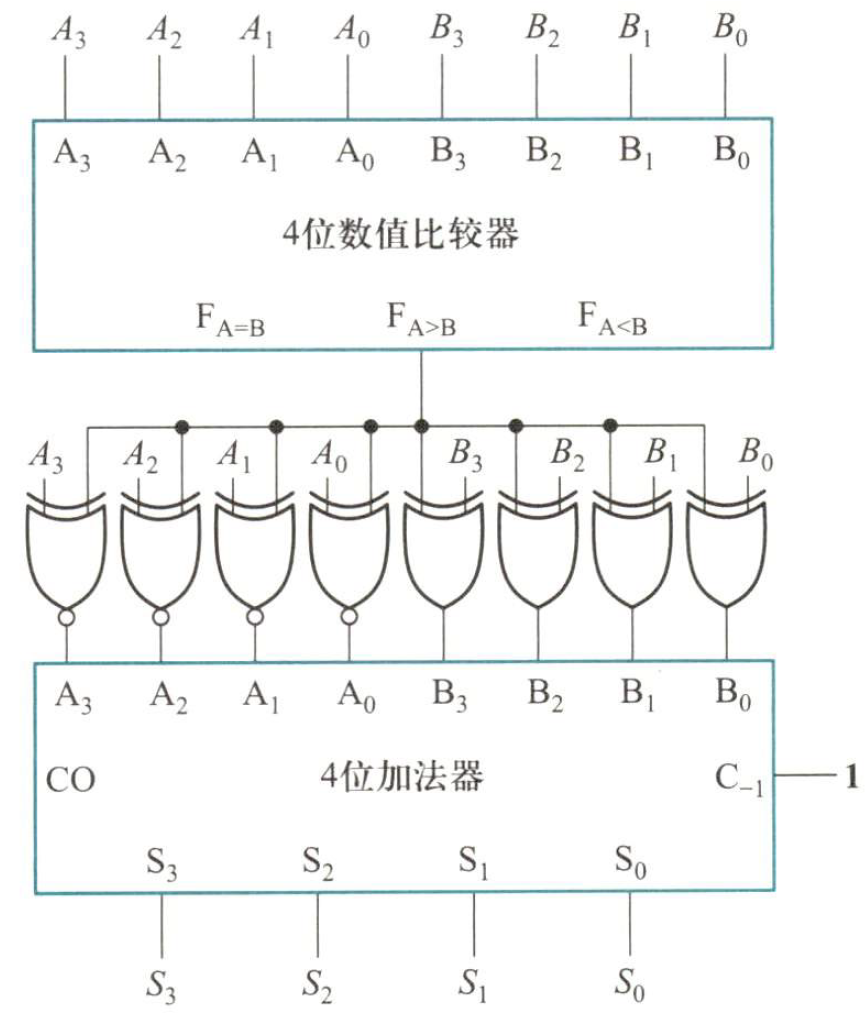
\includegraphics[width=0.5\textwidth]{4.4.37}
	\caption{}
\end{figure}
课堂习题:

(1)一个电路有8个输入信号I7~I0 ,8个输入按键K7~K0,2个输出信号L0和L1。

(2)按键K7~K0用于从8个输入信号I7~I0中选择2个信号从L0和L1中输出。K7按下时17将输出,...,K0按下时10将输出。

(3)按键优先级从高到低为K7~K0。按键高电平有效。

(4)按键每次至少按下任意2个,将优先级最高按键所选择的信号输出到L1,优先级次高按键所选择的信号输出到L0。

(5)例如:同时按下K5、K1和K0,K5优先级最高,I5输出到L1 ; K1优先级次高 , I1输出到L0 ;K0优先级最低,I0不输出。

(6)设计要求: 利用8-3编码器CD4532、3-8译码器74HC138、 8-1选择器74HC151以及门电路,完成以上电路功能。各元器件的数量不限。


\end{document}